\documentclass[11pt,a4paper,sans]{article}
\usepackage{geometry}
\usepackage[some]{background}
\usepackage{color}
\usepackage{hyperref}
\usepackage{pdfpages}

\definecolor{titlepagecolor}{cmyk}{1,.60,0,.40}
\graphicspath{ {../images/} }

\backgroundsetup{
	scale=1,
	angle=0,
	opacity=1,
	contents={\begin{tikzpicture}[remember picture,overlay]
		\path [fill=titlepagecolor] (-0.5\paperwidth,7)rectangle (current page.north east);
		\draw [color=white, very thick] (30,0)--(5,0.5\paperheight);
		\draw [color=white, very thick] (5,0)--(10,0.5\paperheight);
		\draw [color=white, very thick] (7,0)--(10,0.5\paperheight);
	\end{tikzpicture}}
}

\begin{document}
\begin{titlepage}
\BgThispage
\newgeometry{left=1cm,right=1cm,bottom=2cm}
\vspace*{0.1\textheight}
\noindent
\textcolor{white}{\Huge\textbf{\textsf{STORM Project Proposal}}}
\vspace*{4cm}
\noindent
\begin{center}
			\textsc{Clients:} {\huge Linda Marshall \& Vreda Pieterse} \\
			\vspace*{0.3cm}
			\textsc{Proposed by:} {\huge CodingInfinity} \\
			\vspace*{0.1cm}
			\small Department of Computer Science, University of Pretoria \\
			\hfill
\end{center}
\vspace*{1.5cm}
\begin{minipage}{0.35\linewidth}
		\begin{center}
			\textsc{\textbf{Team Members}}
		\end{center}
    \begin{flushright}
        \begin{flushright}
	Andrew Broekman		\emph{11089777}		\newline
	Brenton Watt 		\emph{14032644} 	\newline
	Reinhardt Cromhout 		\emph{14009936} 	\newline
\end{flushright}

    \end{flushright}
\end{minipage} \hspace{15pt}
\begin{minipage}{0.02\linewidth}
    \rule{1pt}{140pt}
\end{minipage} \hspace{-10pt}
\begin{minipage}{0.63\linewidth}
\vspace{5pt}
	\begin{abstract}
		Lecturers of the department of Computer Science at the University of Pretoria, require a system to be developed to shuffle teams. The system is going to be used by the lecturers of the Software Engineering module (COS301) to determine teams for the “Rocking the boat” exercise of the Software Engineering module using a set of lecturer defined criteria to select the teams.
	\end{abstract}
\end{minipage}

\vspace*{1cm}
{\large Date of Submission:} \today
\vfill
\begin{minipage}{\linewidth}
	\begin{center}
		\includegraphics[scale=0.3]{UP_Logo}
	\end{center}
\end{minipage}
\end{titlepage}
\restoregeometry

\pagebreak
\tableofcontents

\pagebreak
\thispagestyle{empty}
\newgeometry{left=7.5cm}
\pagecolor{titlepagecolor}
{\color{white}
\noindent
\textbf{\textsf{\huge The Team}}\\
\makebox[0pt][l]{\rule{1.3\textwidth}{1pt}}}
\restoregeometry
\nopagecolor
\includepdf[]{BrentonStandard.pdf}
\includepdf[]{reinhardtStandard.pdf}
\includepdf[]{fabioStandard.pdf}


\pagebreak
\thispagestyle{empty}
\newgeometry{left=7.5cm}
\pagecolor{titlepagecolor}
{\color{white}
\noindent
\textbf{\textsf{\huge Project Execution}}\\
\makebox[0pt][l]{\rule{1.3\textwidth}{1pt}}}
\restoregeometry
\nopagecolor
\section{Project Execution}
\subsection{Development Methodology}
The CodingInfinity team will be using the \textbf{Agile Software Development methodology} during the course of the project. Agile Software Development is an umbrella term used to refer to the values and principels expressed in the Agile Manifesto.

In particular we find value in the following four points:
\begin{itemize}
	\item \textbf{Individuals and interactions} over processes and tools.
	\item \textbf{Working software} over comprehensive documentation.
	\item \textbf{Customer collaboration} over contract negotiation.
	\item \textbf{Responding to change} over following a plan.
\end{itemize}

Although we find value in the items on the right, we value the items on the left, emphasised in bold, even more.

The Agile princples themselves are derived from the following twelve principles:
\begin{itemize}
  \item Customer satisfaction by early and continuous delivery of valuable software
  \item Welcome changing requirements, even in late development
  \item Working software is delivered frequently (weeks rather than months)
  \item Close, daily cooperation between business people and developers
  \item Projects are built around motivated individuals, who should be trusted
  \item Face-to-face conversation is the best form of communication (co-location)
  \item Working software is the principal measure of progress
  \item Sustainable development, able to maintain a constant pace
  \item Continuous attention to technical excellence and good design
  \item Simplicity—the art of maximizing the amount of work not done—is essential
  \item Best architectures, requirements, and designs emerge from self-organizing teams
  \item Regularly, the team reflects on how to become more effective, and adjusts accordingly
\end{itemize}

Agile development seeks to provide opportunities to assess the changing functional and technical landscape while maintaining focus on rapid and continous delivery of business value. This results in decreased overall risk associated with software development.

A core focus in Agile software development is to ensure that value is continously derived throught the developement lifecycle, which is achieved through a process of continuous planning and feedback. This process creates a feedback loop ensuring that the delivered software can be continuously aligned with the desired business needs and creates the opportunity for easy adaption to changing requirements throughout the process.

With continuous monitoring and measuring of the project status through continuous testing the client gains much more visibility into and around the actual progress of the project.

As a result of following an Agile Development approach the final deliverable software system will be able to much better address the business and customer needs than what would have produced with alternative methodologies.

\begin{figure}[t]
  \centering
  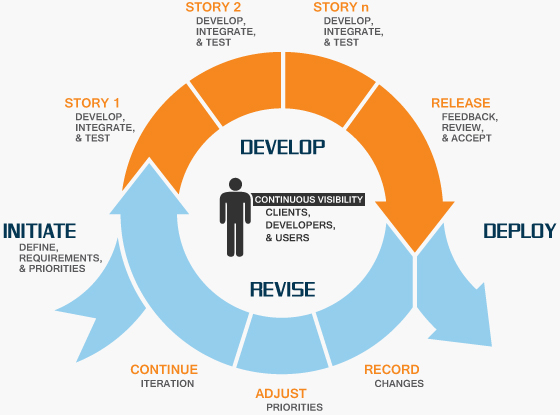
\includegraphics[width=175px]{agile.jpg}
\end{figure}


\subsection{Informing the Client}
\begin{itemize}
	\item Since the client is on site we will want to have weekly meetings where we will report on what has been done in the past week and suggest and discuss what will be done in the coming week. This is also in line with die aglie development methodology that has been chosen.
	\item Email will be used if the team has questions for the client that can not wait until the next meeting.
	\item The client may potentially have access to a scrum server the developers are using for the project.
\end{itemize}

\subsection{Initial Ideas on Solving Some Technical Challenges}
\begin{itemize}
	\item 
\end{itemize}

\subsection{Technologies We will Use}
\begin{itemize}
	\item Spring
	For dependancy injection and Aspect Oriented Programming.
	\item Java
	For the main development of the backend, allthough for the actual benchmarking a lower level language like C++ might be considered to do measurements. This is so that the programs are executed by a language that does not run through something like the Java VM.
	\item AngularJS
	\item This will be combined into a microservices architecture
\end{itemize} 

\subsection{What Will The Client Receive}
On completion of the development cycle the client will receive the following:
\begin{itemize}
	\item The functional application, which includes:
	\begin{itemize}
		\item The functioning web interface
		\item The backend which will run the bechmarking tests and record the results
	\end{itemize}
	\item The source code for the functional application
	\item Associated build files
	\item The source code for all unit and integration tests
	\item The full spesification documentation as required by the agile development methodology
	\item (possibly) a simple user manual, but this will be debated since part of the goals of the project are to develop a generic, easy to use benchmarking system that the user can hopefully use without much training
\end{itemize}


\end{document}
